% Write the paper here, and submit from here. The target journal, the suggested
% reviewers and the table of contents below are for internal circulation; the
% generator strips them, so they never reach a journal.
\documentclass[12pt,a4paper]{article}
\usepackage{authblk}
\usepackage{fullpage}
\usepackage{amssymb,amsmath}
\usepackage[utf8x]{inputenc}
\usepackage[T1]{fontenc}
\usepackage{siunitx}
\usepackage{isomath}

\usepackage[left]{lineno} % line numbers
\modulolinenumbers[5]     % print every fifth one; lineno still counts every line

\usepackage{setspace}
\doublespacing

\usepackage[unicode=true]{hyperref}
\hypersetup{breaklinks=true,
            bookmarks=true,
            colorlinks=false,
            pdfborder={0 0 0}}
\urlstyle{same}

\setcounter{secnumdepth}{5}

\usepackage{graphicx}
\usepackage[super, numbers, sort&compress]{natbib}

% Highlighting for internal review.
\usepackage{xcolor}
\usepackage{soul}
\definecolor{reviewyellow}{rgb}{1, 1, 0.6}
\sethlcolor{reviewyellow}

%%%%%%%%%%%%%%%%%%%%%%%%%%%%%%%%%%%%%%%%%%%%%%%%%%%%%%%%%%%%%%%%%%%%%%%%%%%%%%

\title{ \bfseries Working Title of the Paper}
\author[a]{First Author}
\author[b]{Second Author}
\author[a]{Third Author}

\renewcommand\Affilfont{\small\itshape}
\affil[a]{First Institute, First University, Country}
\affil[b]{Second Institute, Second University, Country}

\date{}

%%%%%%%%%%%%%%%%%%%%%%%%%%%%%%%%%%%%%%%%%%%%%%%%%%%%%%%%%%%%%%%%%%%%%%%%%%%%%%


% Tracked changes for the revision (see https://ctan.org/pkg/changes).
% This file is the annotated version, so the changes stay visible. The clean
% version is produced by scripts/prepare_submission.py, which accepts them.
\usepackage{changes}
\definechangesauthor[color=blue]{R1}
% ulem-based underline/strikeout breaks around superscript \cite, so use plain markup
\setaddedmarkup{#1}
\setdeletedmarkup{\textcolor{gray}{[deleted: #1]}}

\begin{document}

\maketitle

\newpage

\linenumbers

\section*{Abstract}
\linelabel{ln:abstract}\replaced{The revised opening sentence}{An earlier phrasing}. \added{A sentence added for a reviewer.}
State the gap in the first two sentences, the approach in the middle, and the
headline result at the end \cite{firstReference2024}. Keep it to the word limit of
the target journal.

\section*{Synopsis}
Two sentences on why this matters beyond the immediate field, if the target
journal asks for a synopsis or significance statement.

\section*{Keywords}
first keyword, second keyword, third keyword, fourth keyword

% No caption, so the graphical abstract takes no figure number of its own.
\begin{figure}[!ht]
    \centering
    \noindent
    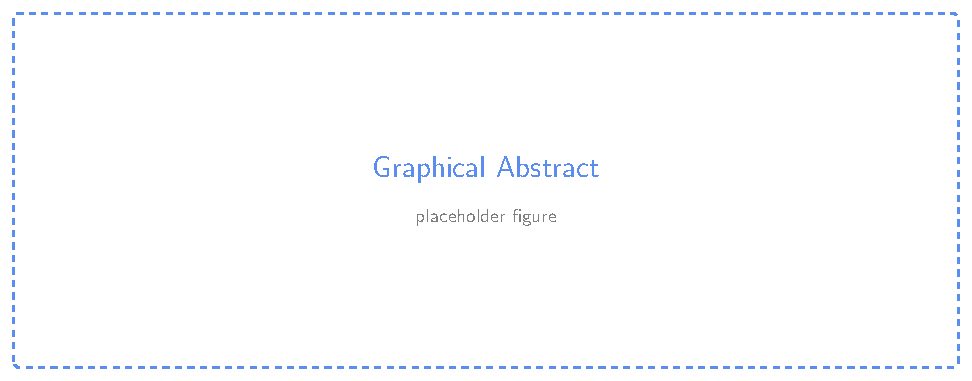
\includegraphics[width=\textwidth]{figs/graphical_abstract.pdf}
\end{figure}

\section*{\hl{Target Journal: Name of the Journal}}

\section*{\hl{Reviewer Suggestions}}

\begin{itemize}
    \item \hl{First Suggested Reviewer --- Institution, Country}
    \item \hl{Second Suggested Reviewer --- Institution, Country}
    \item \hl{Third Suggested Reviewer --- Institution, Country}
\end{itemize}

\newpage

\tableofcontents
\newpage

%%%%%%%%%%%%%%%%%%%%%%%%%%%%%%%%%%%%%%%%%%%%%%%%%%%%%%%%%%%%%%%%%%%%%%%%%%%%%%

\section{Introduction}

Open with the wider context and narrow towards the specific gap this paper
closes \cite{firstReference2024, secondReference2023}. One paragraph per step of
that narrowing usually suffices.

\linelabel{ln:gap}State what remains unresolved, and why the existing approaches cannot resolve it
\cite{thirdReference2022}. Be concrete about the limitation rather than listing
papers. Where a study is the subject of the sentence, name it instead, as
\citet{secondReference2023} did.

Close the introduction by saying what this work does, in the order the rest of
the paper presents it. Several references at once compress into a range
\cite{firstReference2024, secondReference2023, thirdReference2022}.

%%%%%%%%%%%%%%%%%%%%%%%%%%%%%%%%%%%%%%%%%%%%%%%%%%%%%%%%%%%%%%%%%%%%%%%%%%%%%%

\section{Methods} \label{sec:methods}

Describe the approach so that someone else could repeat it. Introduce notation
once and use it consistently. Let $\vectorsym{x}$ denote the vector of decision
variables and $\matrixsym{A}$ the coefficient matrix, so that

\begin{equation} \label{eq:example}
    \matrixsym{A} \, \vectorsym{x} = \vectorsym{b},
\end{equation}

where $\vectorsym{b}$ is the demand vector. Refer back to
Eq.~\ref{eq:example} rather than repeating it.

\subsection{First Component} \label{sec:first_component}

Split the methods into the components a reader needs in order. Each subsection
should answer one question.

\subsection{Second Component}

Where a figure explains the structure better than prose does, use one.

\begin{figure}[!ht]
    \centering
    \noindent
    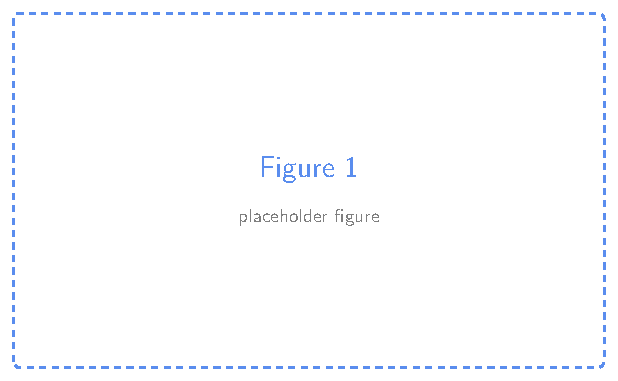
\includegraphics[width=0.6\textwidth]{figs/figure_one.pdf}
    \caption{Caption stating what the figure shows and what to take from it.}
    \label{fig:figure_one}
\end{figure}

\subsection{Implementation}

Name the software, the versions, and where the code lives. Point at the
documentation rather than reproducing it.

%%%%%%%%%%%%%%%%%%%%%%%%%%%%%%%%%%%%%%%%%%%%%%%%%%%%%%%%%%%%%%%%%%%%%%%%%%%%%%

\section{Results} \label{sec:results}

Set up the case or dataset first, then report what it produced. Quantify by stating
the number, its unit, and what it should be compared against.

\begin{figure}[!ht]
    \centering
    \noindent
    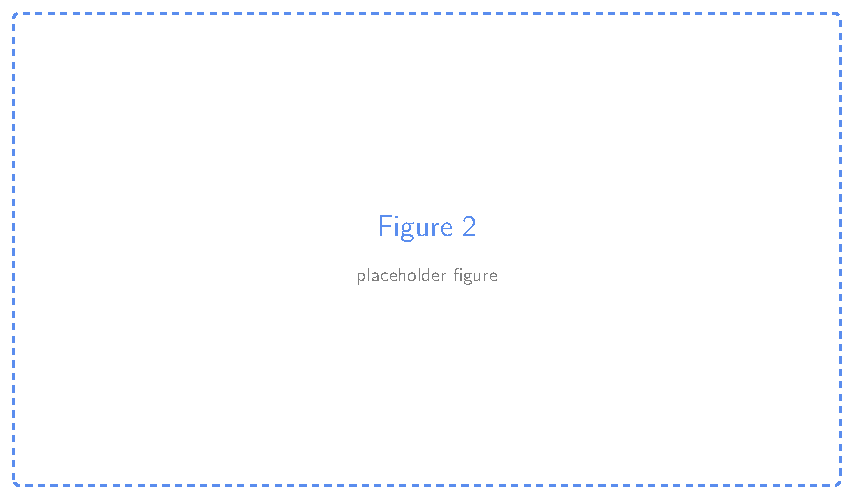
\includegraphics[width=\textwidth]{figs/figure_two.pdf}
    \caption{Caption stating what the figure shows and what to take from it.}
    \label{fig:figure_two}
\end{figure}

Walk through Fig.~\ref{fig:figure_two} in the order a reader meets it, and say
what each panel establishes.

%%%%%%%%%%%%%%%%%%%%%%%%%%%%%%%%%%%%%%%%%%%%%%%%%%%%%%%%%%%%%%%%%%%%%%%%%%%%%%

\section{Discussion} \label{sec:discussion}

Say what the results mean for the gap identified in the introduction, without
restating them.

\subsection{Limitations}

State the assumptions that would change the conclusions if violated, and how far
they can be relaxed.

\subsection{Outlook}

Name the concrete next steps this work makes possible.

%%%%%%%%%%%%%%%%%%%%%%%%%%%%%%%%%%%%%%%%%%%%%%%%%%%%%%%%%%%%%%%%%%%%%%%%%%%%%%

\newpage\clearpage

\renewcommand\refname{References}
\bibliographystyle{unsrtnat}
\bibliography{../references}
\newpage

\end{document}
